\chapter{Clean Architecture}

\section{Was ist Clean Architecture?}
Die Clean Architecture ist eine Richtlinie für das Programmieren von Software. Dabei wird die Codebasis in 4 Schichten aufgeteilt:
\begin{itemize}
	\item \textbf{Plugin Schicht:} Diese Schicht enthält sämtlichen Framework oder Gerät abhängigen Code
	\item \textbf{Adapter Schicht:} Diese Schicht enthält jeglichen Code, der Daten / Methoden der Plugin Schicht, zur Nutzung der Unteren Schichten umformt. Sie stellt also sicher, das die unteren Schichten Fehlerfrei verwendet werden können.
	\item \textbf{Application Schicht:} Die Applikationsschicht enthält alle Use-Cases der Applikation und repräsentiert somit alle möglichen und verfügbaren Aktionen die die Applikation abbildet. Sie enthält ausschließlich Business Logik und weiß nicht wer den Code Ausführt, noch wie er am Ende präsentiert werden soll.
	\item \textbf{Domain Schicht:} Diese Schicht enthält alle Objekte die die Anwendungsdomaine repräsentieren.
\end{itemize}
Wichtig ist, das eine äußere Schicht abhängig von einer inneren Schicht sein darf, eine innere Schicht allerdings nicht von einer äußeren Schicht. Das ist die sogennante \enquote{Dependency Rule}. Damit wird der primäre Zweck der Clean Architecture sichergestellt: Das ordnen von Code nach zeitlicher relevanz und das ermöglichen von einfachem Austauschen von kurzfristigem Code. Durch diese Architektur, lassen sich Frameworks oder Persistierungsimplementation jederzeit schnell und einfach austauschen, während der gültige Domaincode nicht verändert werden muss. Somit muss der Kern einer Applikation nur einmal geschrieben werden, während man sie auf beliebige Art und Weise bereitstellen kann.

\section{Analyse der Dependency Rule}
[(1 Klasse, die die Dependency Rule einhält und eine Klasse, die die Dependency Rule verletzt);   jeweils UML der Klasse und Analyse der Abhängigkeiten in beide Richtungen (d.h., von wem hängt die Klasse ab und wer hängt von der Klasse ab) in Bezug auf die Dependency Rule]

\subsection{Positiv-Beispiel: Dependency Rule}
\begin{figure}[H]
	\centering
	\includegraphics[width=0.9\textwidth]{Bilder/RollIniView.pdf}
	\caption{UML RollDiceService}
	\label{fig:RollDiceServiceDependencys}
\end{figure}
Abbildung \ref{fig:RollDiceServiceDependencys} das UML Diagramm der Klasse \texttt{DiceRollService}. Diese Klasse ist teil des Application Layers der Clean Architecture und darf somit nur von unteren Layern abhängen. Wie der Abbildung zu entnehmen ist, ist dies der Fall. Die Klasse hängt ausschließlich von den Klassen \texttt{HitDie}, \texttt{HitDieException}, \texttt{Weapon}, \texttt{DiceRollException} und \texttt{RPGCharacter} ab. All diese Klassen liegen in der Domain Schicht. Abhängig von der Klasse \texttt{DiceRollService} sind die Klassen \texttt{RollSkill}, \texttt{RollSavingThrow}, \texttt{RollIniView}, \texttt{CheckView} und \texttt{RollAttack}, die in der Plugin Schicht liegen und teil des User-Interfaces sind. Somit wird die Dependency Rule bei dieser Klasse eingehalten.


\subsection{Negativ-Beispiel: Dependency Rule}
Aus älterem Commit die Repository Implementation

\section{Analyse der Schichten}

\subsection{Plugin: MainMenu}
\begin{figure}[H]
	\centering
	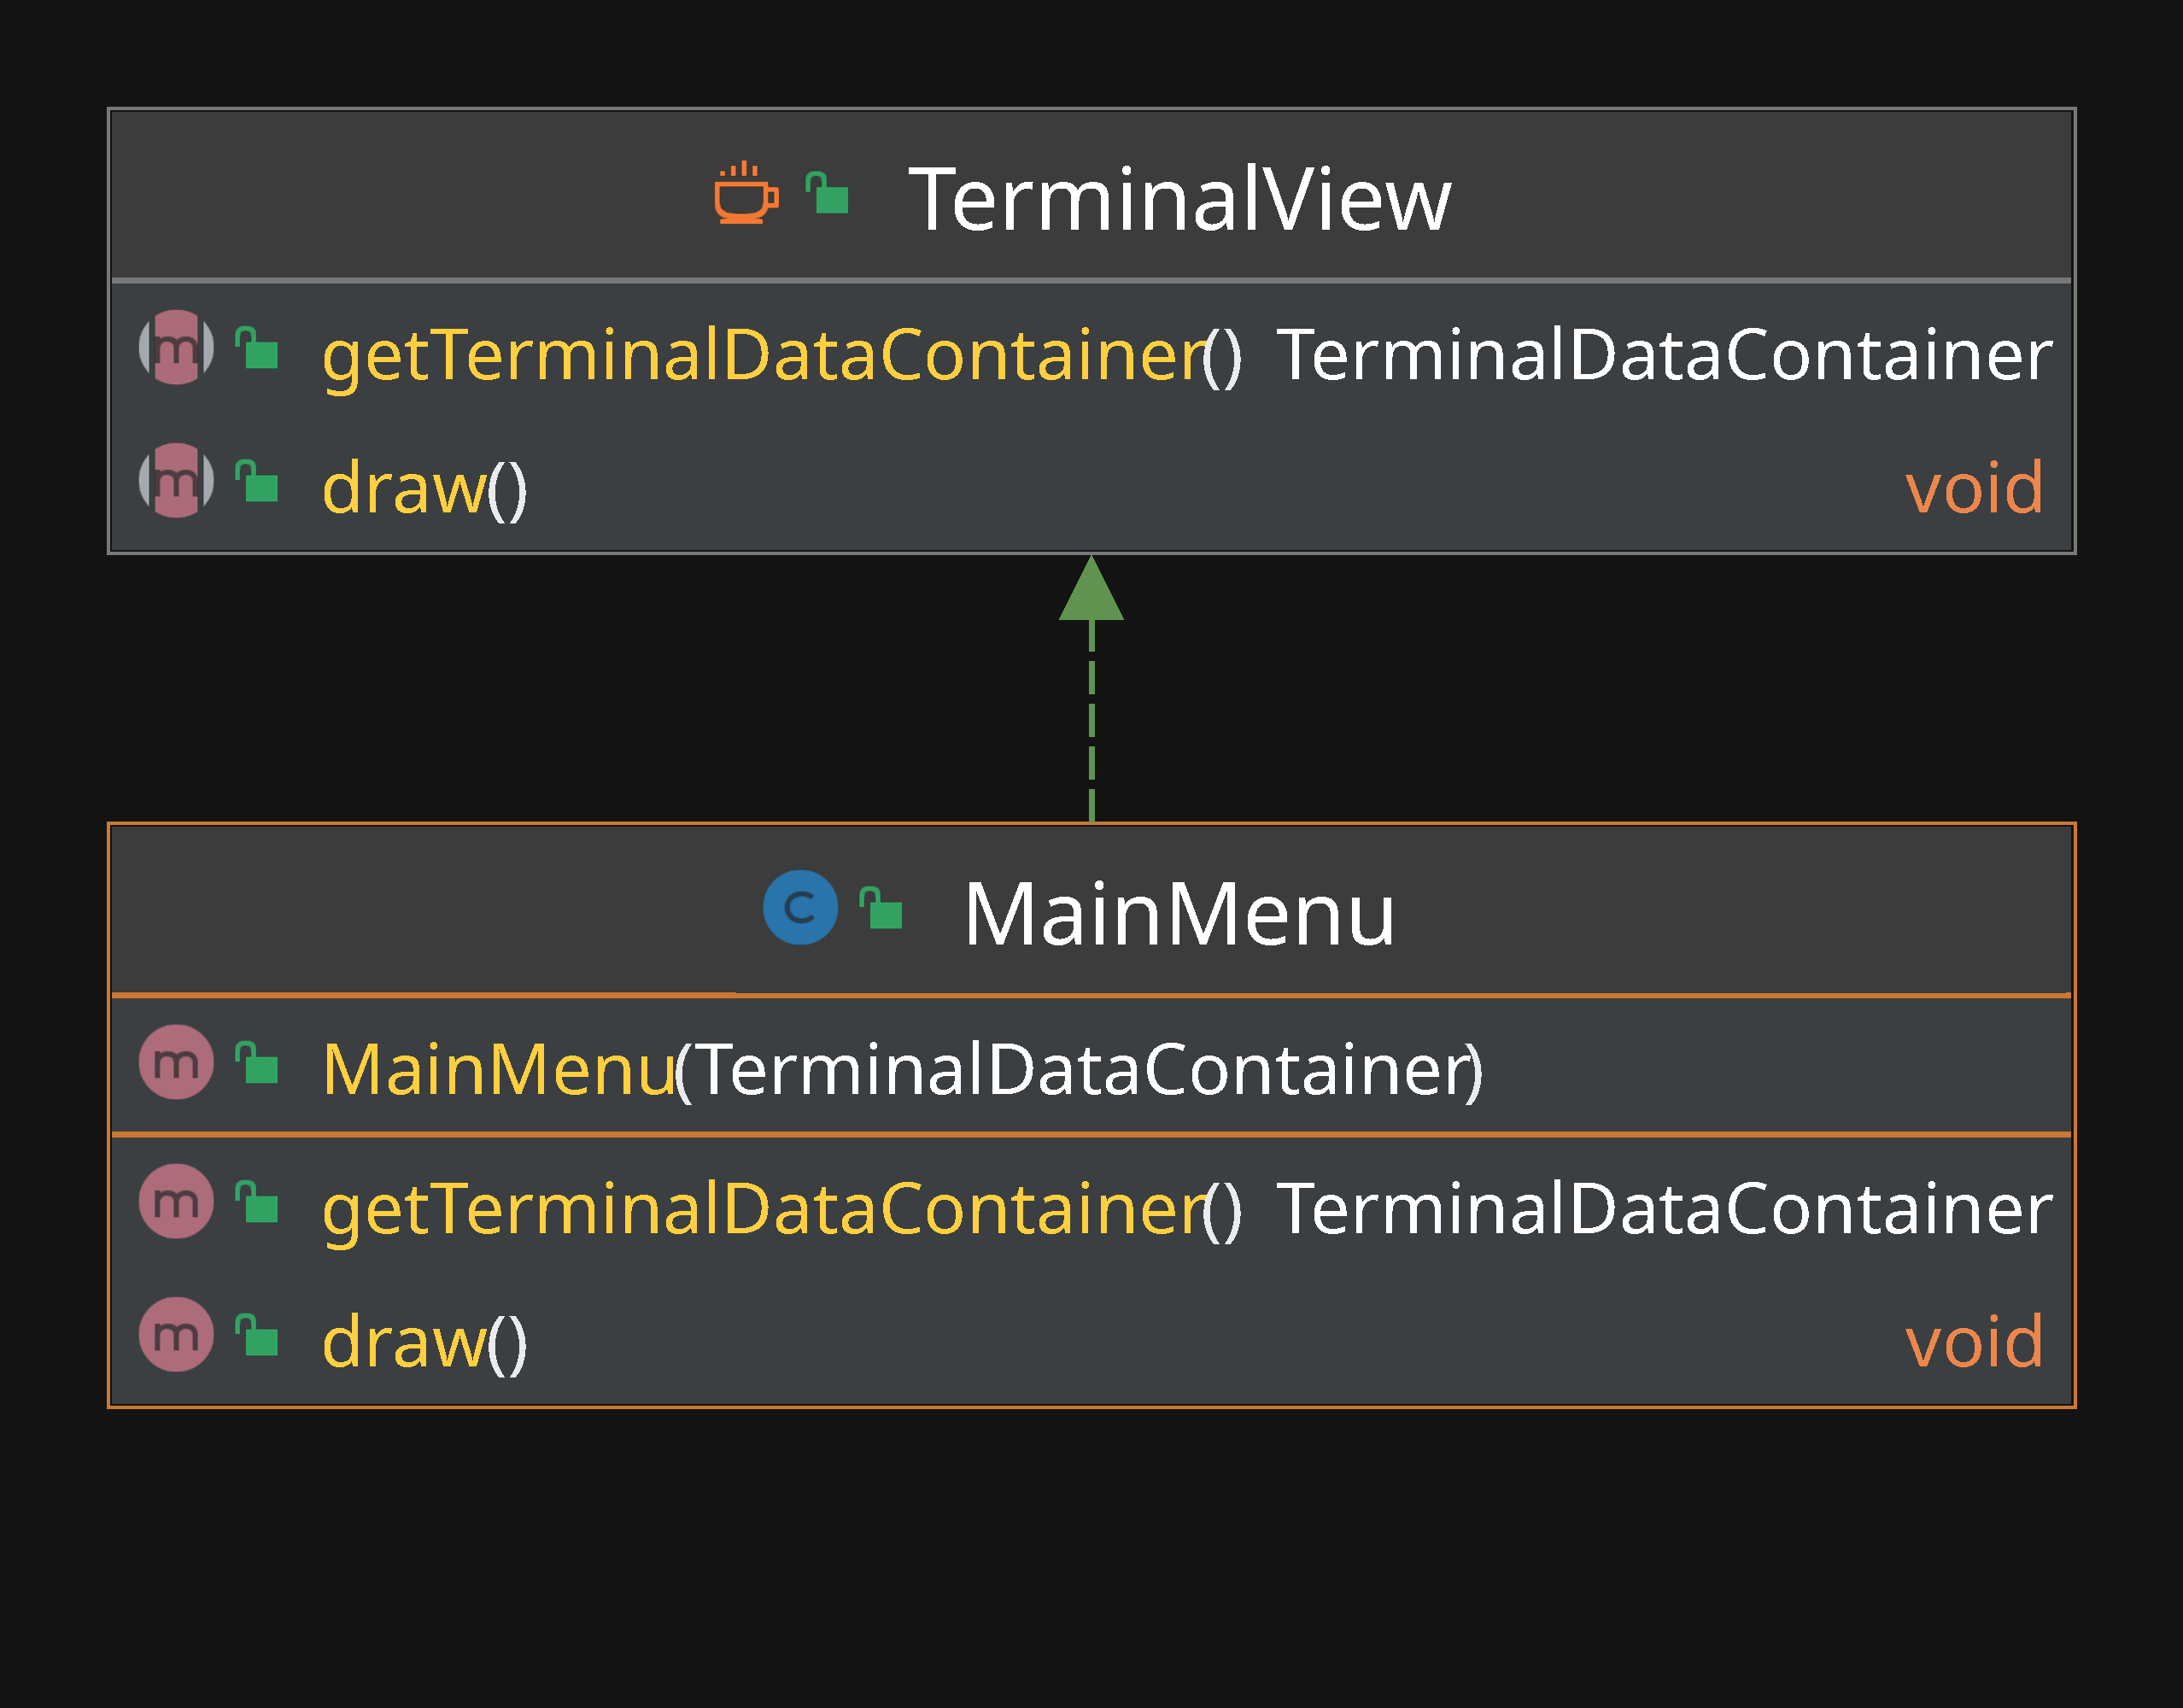
\includegraphics[width=0.5\textwidth]{Bilder/MainMenu.pdf}
	\caption{UML MainMenu}
	\label{fig:MainMenu}
\end{figure}

Die Klasse \texttt{MainMenu} liegt in der Plugin Schicht, da sie Teil des User Interfaces ist. Sie stellt den Einstiegspunkt der Nutzer Interaktion dar und stellt alle Möglichkeiten und Navigationspunkte dem User dar. Da die Implementierung des User Interfaces Framework spezifisch, bzw. Gerät spezifisch ist, gehört diese Klasse klar in die Plugin Schicht der Clean Architecture. Abbildung \ref{fig:MainMenu} zeigt das UML der Klasse.

\subsection{Domain: Weapon}
\begin{figure}[H]
	\centering
	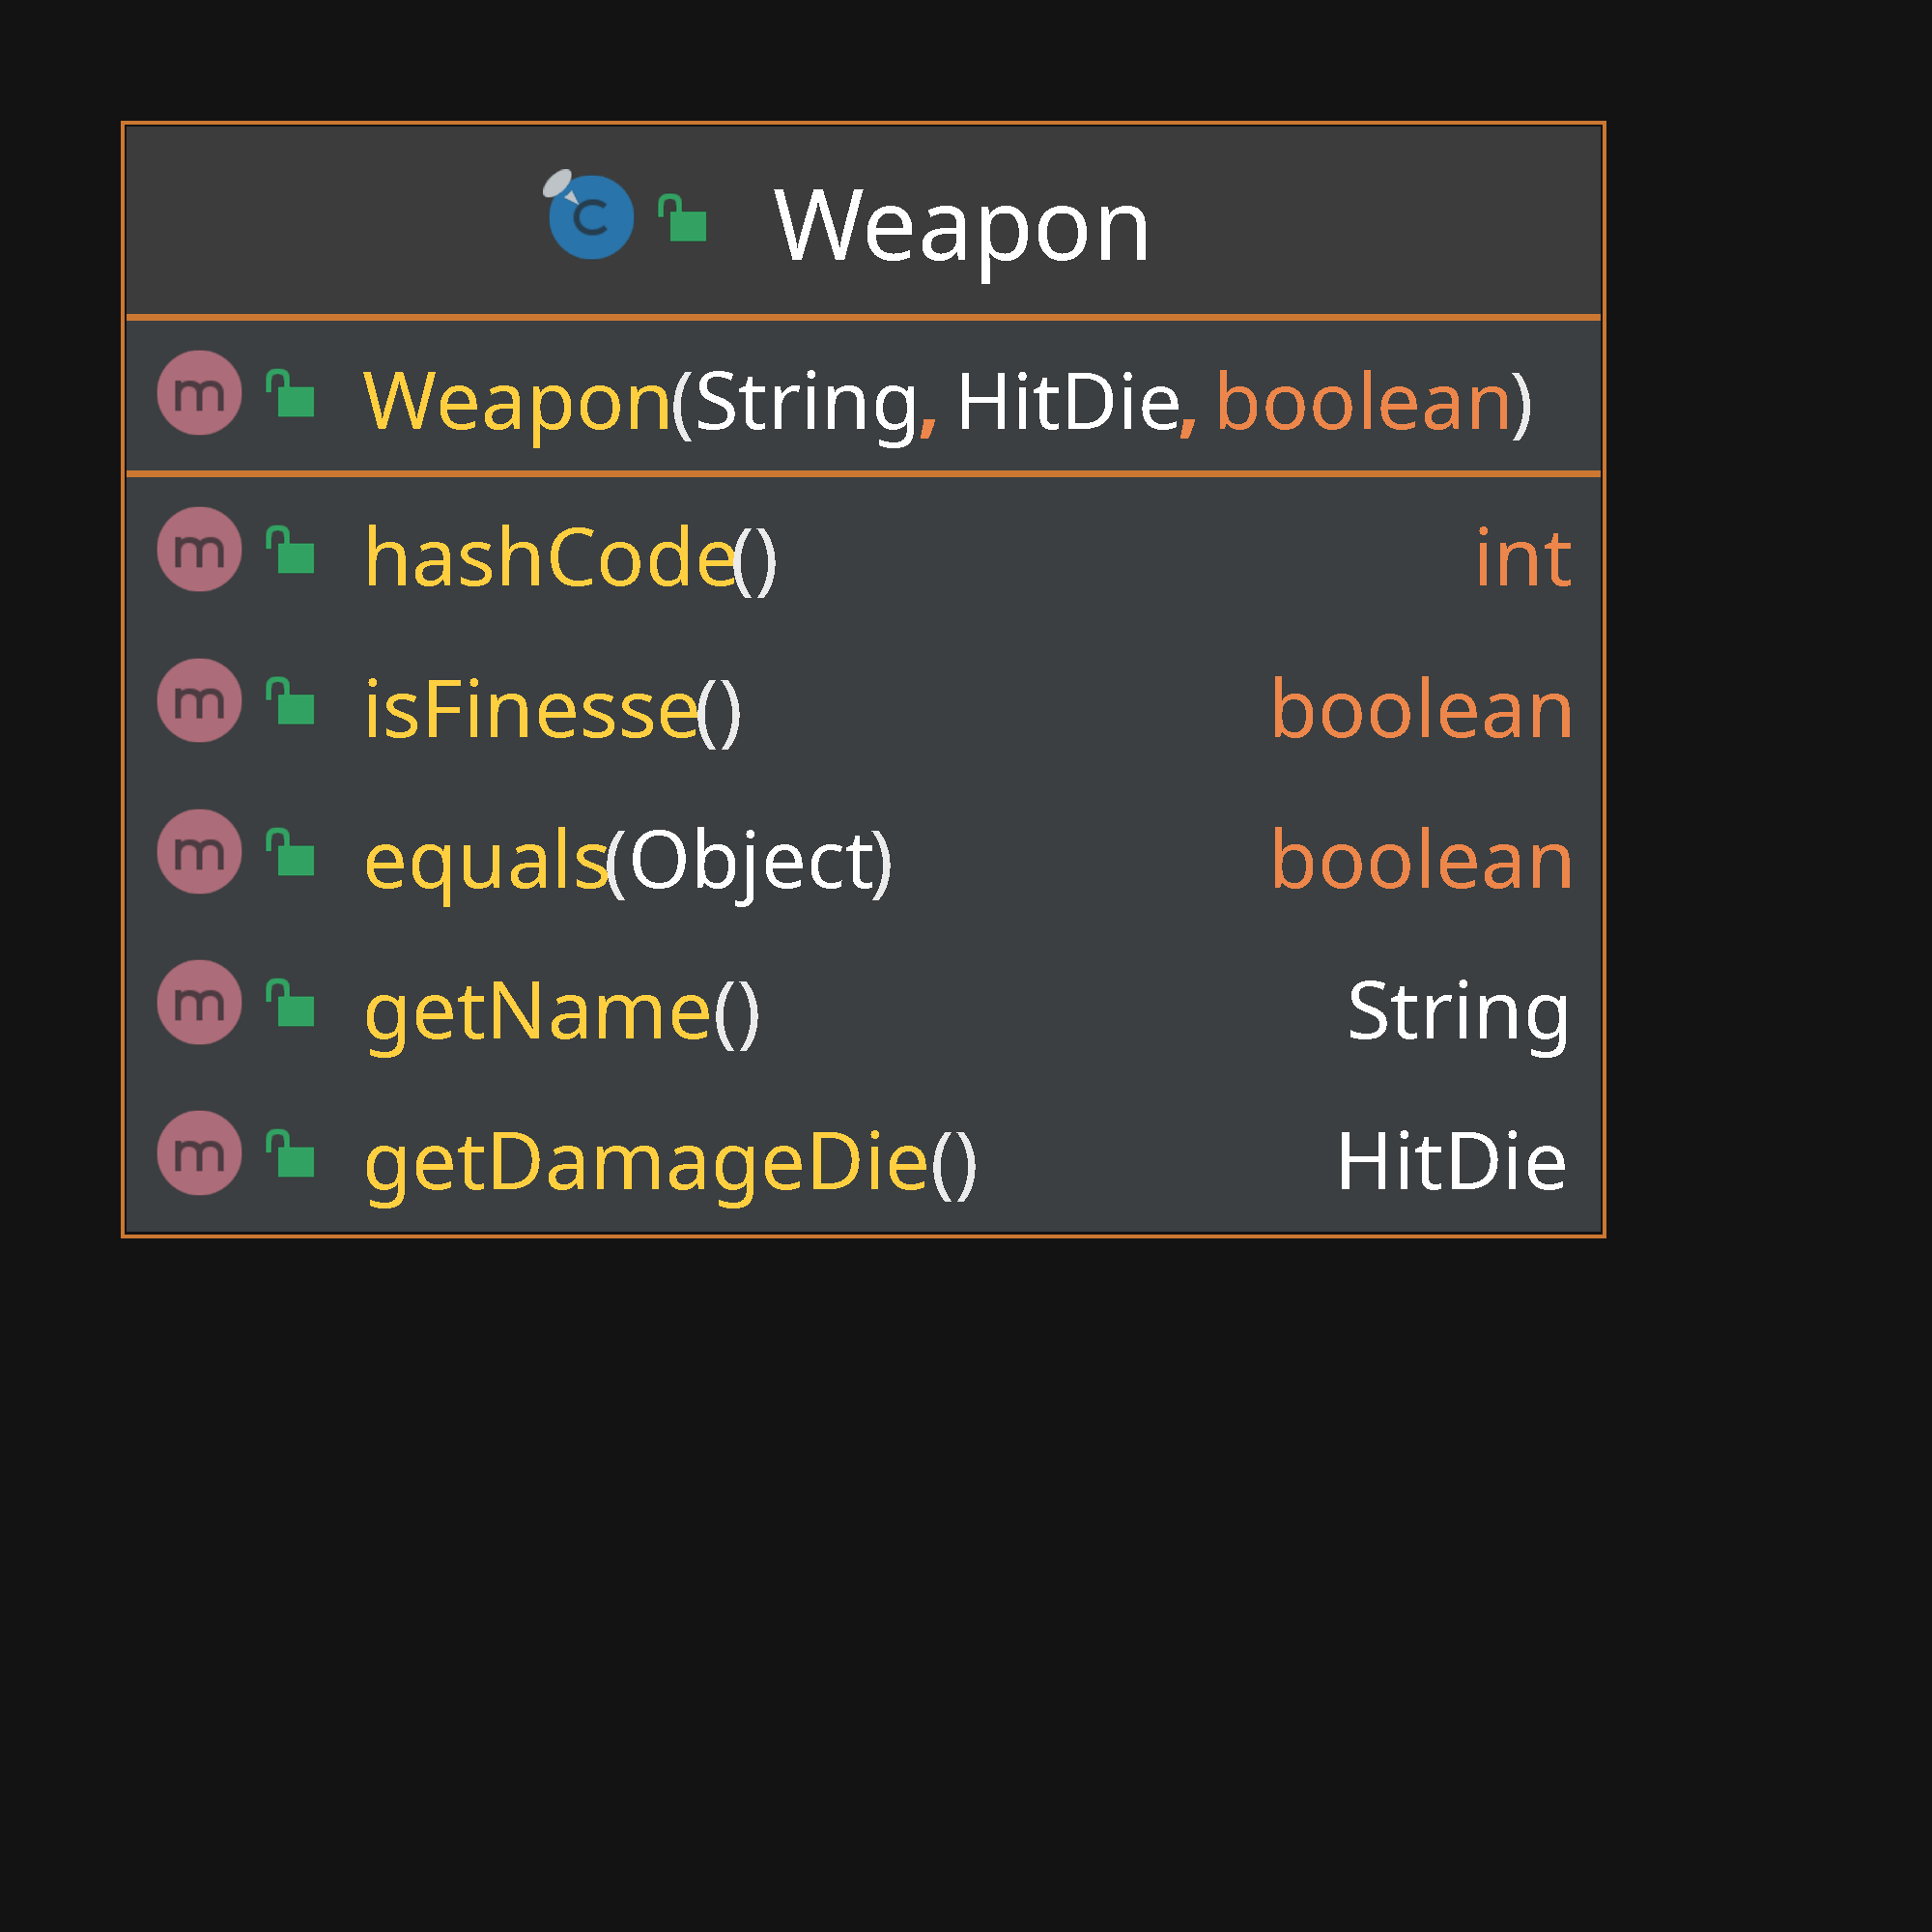
\includegraphics[width=0.5\textwidth]{Bilder/Weapon.pdf}
	\caption{UML Weapon}
	\label{fig:Weapon}
\end{figure}
Die Klasse Weapon Modelliert eine Waffe aus D\&D 5e. Sie enthält ausschließlich Daten und modelliert einen wichtigen Teil der Anwendungsdomaine. Somit ist sie klar in die Domain Schicht der Clean Architecture einzuordnen.
